\chapter{Word2Vec}\label{word2vec}

In diesem Kapitel wird das Verfahren "Word2Vec" durch die Nutzung von neuronalem Netz vorgestellt. Word2Vec ist eine Darstellung von Wörtern mit Vektoren, was auch die Abkürzung erklärt. \textit{Word} steht für \textit{Wort}, \textit{2} steht für \textit{to}, also zu, und \textit{Vec} steht für \textit{Vector}. Diese Wortrepräsentation wird in der Natural Laguage Processing (NLP) benutzt und findet Anwendung in Bereichen wie Spamfilterung und Dokumentenanalyse. Jedoch erklärt diese Technik nur, wie die Wörter eines Textes dargestellt werden können. Das Verfahren, bei dem die möglichst passenden Vektoren in einem ausgewählten Text, auch Corpus genant, gelernt werden, heißt Word Embedding. Bei dieser Technik wird ein neuronales Netz eigesetzt. Die Vorgehensweise und die Idee wird folglich erklärt.

\section{Word Embedding}

Wie bereits in der Einleitung erwähnt wurde, ist Word Embedding ein Prozess, bei dem die Wörter eines Textes in Vektoren umgewandelt werden. 

%Zuerst muss der Corpus vorbeiretet werden. Ich stelle hier nur die Theorie und in einer späteren Kapitel (!? WICHTIG WELCHE GENAU!?) gehe ich tiefer in dem Programmcode.
%
%\!!! DAS HIER GEHÖRT IN EINE ANDERE KAPITEL !!!
%!!! DIE KAPITEL FÜR TEXTVORBEREITUNG ODER SOWAS!!!
%
%Als der Text vorbeitet ist, sodass es von Sonderzeichen und alle unnötigen Zeichen bereinigt wird. Wenn der Text vorbeireitet ist, werden die Wörter aus dem Corpus bestimmt und jeder erhält einen Index. Üblicherweise werden die Wörter nach ihrer Häufigkeit angeordnet. Das häufigste Wort erhält somit den Index 1. Als nächstes werden die Wörter im Corpus durch ihren Index ersetzt, um alle Trainingspaare fürs Lernen generiert zu werden. Dies erfolgt in dem es durch das Corpus iteriert und in einem bestimmten Fenster, oder in der Literatur auch als Window gezeichnet, alle Contextwörter und den Targetwort ausgelesen werden. Das Targetwort ist das Wort in der Mitte, während die Wörter um das Targetwort entsprechend die Kontextwörter. 
%
%!!! BIS HIER MUSS WEG !!!!

In der Literatur spricht man von zwei Arten von Wort2Vec Methoden - SKIP-gram und CBOW (Continous Bag of Words) \cite{Ali:19}. Beide Verfahren verwenden ein neuronales Netz. Die beiden Methoden unterscheiden sich nach ihren Ein- und Ausgaben.   

\subsubsection{SKIP-gram Model}
Bei dem SKIP-gram-Modell fließen die Targetwörter als Eingabe und das Modell versucht ein Kontextwort zu raten. Hier ist die Struktur eines Skip-gram Modells gegeben \cite{Ali:19}:

\begin{figure}[H]
	\centering
	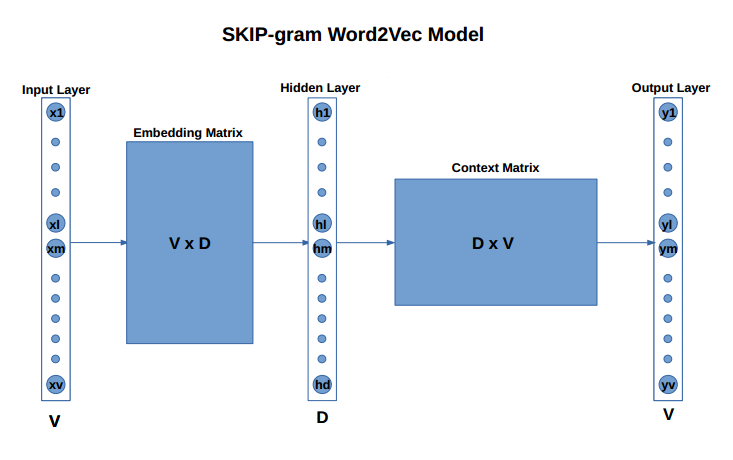
\includegraphics[scale=0.6]{images/SKIP_Model.png}
	\caption{Skip-gram Word2Vec Model}
	\label{skip}
\end{figure}

Der Abbildung \ref{skip} ist zu entnehmen, dass ein Skip-gram Modell aus einer versteckten Schicht, eine Ein- und eine Ausgabeschicht besteht. Die Eingabe sowie die Ausgabe ist ein Vektor, der aus $\emph{V}$ Komponenten besteht. $\emph{V}$ entspricht der Größe des Wörterbuchs (engl. Vocabulary). Die versteckte Schicht besteht aus $\emph{D}$ Variablen und stellt einen Vektor dar. $\emph{D}$ nimmt üblicherweise einen Wert zwischen 25 und 300. Diese Variablen können auch als Eigenschaften für die Wörter betrachtet werden. Je mehr Kriterien untersucht werden, desto besser können die Beziehungen zwischen den Wörtern dargestellt werden. Die Ausgabe ist wieder ein $\emph{V-dimensionaler}$ Vektor. Jedoch ist die Ausgabe kein One-Hot Vektor mehr, sondern ein Wahrscheinlichkeitsvektor, der die Wahrscheinlichkeiten für jedes Wort aus dem Corpus beinhaltet.

Die zwei Matrizen sind identisch, jedoch ist die Kontextmatrix die transponierte Embeddingsmatrix (\cref{skip}). In der Matrix sind unsere Wortvektoren zu finden.

Die Multiplikation der Eingabe mit der Embedding-Matirx liefert den ausgeblendeten Schichtvektor. Eine weitere Multiplikation mit der Context-Matrix berechnet wiederum die Ausgabe.

\subsubsection{CBOW Model}
Umgekehrt fließen bei dem CBOW-Model die Kontextwörter als Eingabe, während das Targetwort geliefert wird. Die zwei Modelle besitzen die gleiche Anzahl an Schichten. Das CBOW-Modell ist ein umgedrehtes SKIP-gram-Modell, jedoch besteht die Eingabe aus $\emph{w}$-Viele Vektoren statt nur einem, wo $\emph{w}$ das Kontextfenster darstellt. Als nächstes stellt \cref{cbow} die beschriebene Struktur dar.

\begin{figure}[H]
	\centering
	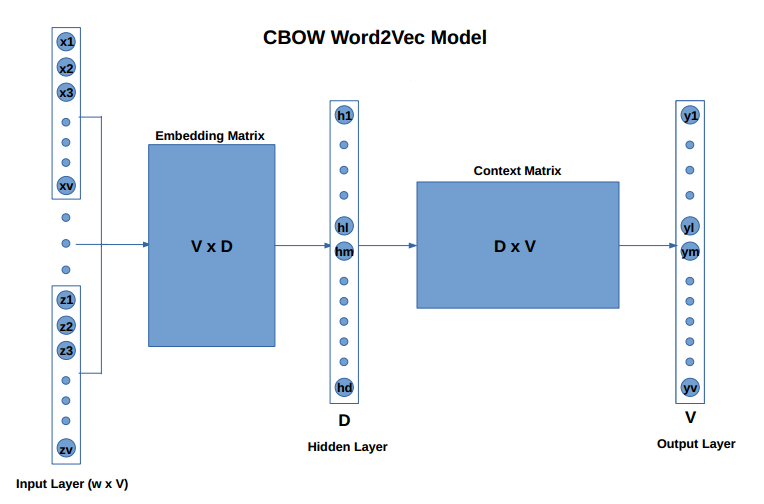
\includegraphics[scale=0.6]{images/CBOW_Model.png}
	\caption{CBOW Word2Vec Model}
	\label{cbow}
\end{figure}

Die Struktur des CBOW-Modells besteht wieder aus einer Matrix für das Embedding der Target- und Kontextwörter. Die Größe der Matrizen hängt von den ausgewählten Hyperparametern und der Größe des Datensatzes ab. Die Anzahl der verwendeten Inputvektoren entspricht der Größe des gesetzten Fensters (Kontextfenster).
